\documentclass[conference]{IEEEtran}
\usepackage{cite}
\usepackage{amsmath,amssymb,amsfonts}
\usepackage{algorithmic}
\usepackage{algorithm}
\usepackage{graphicx}
\usepackage{textcomp}
\usepackage{xcolor}
\usepackage{booktabs}
\usepackage{multirow}
\usepackage{hyperref}
\usepackage{tabularx}
\usepackage{float}
\usepackage{url}

\begin{document}

\title{NyayaSahaya: A Hardware-Integrated Retrieval-Augmented Generation Platform for Democratizing Legal Assistance in India}

\author{
\IEEEauthorblockN{Hemang S Desai}
\IEEEauthorblockA{\textit{Department of Computer Science and Engineering} \\
\textit{RV College of Engineering}\\
Bengaluru, India \\
hshrikardesai.cs23@rvce.edu.in}
\and
\IEEEauthorblockN{Sumadhva Krishna H M}
\IEEEauthorblockA{\textit{Department of Computer Science and Engineering} \\
\textit{RV College of Engineering}\\
Bengaluru, India \\
sumadhvak.cs23@rvce.edu.in}
\and
\IEEEauthorblockN{Sudeep P Hande}
\IEEEauthorblockA{\textit{Department of Electronics and Communication Engineering} \\
\textit{RV College of Engineering}\\
Bengaluru, India \\
sudeepphande.ec23@rvce.edu.in}
\and
\IEEEauthorblockN{Tejasvi Mallaih}
\IEEEauthorblockA{\textit{Department of Electronics and Communication Engineering} \\
\textit{RV College of Engineering}\\
Bengaluru, India \\
tejasvimallaiah.ec23@rvce.edu.in}
\and
\IEEEauthorblockN{Dr.~Vinay Hegde}
\IEEEauthorblockA{\makebox[\linewidth][c]{\textit{Department of Computer Science and Engineering}} \\
\makebox[\linewidth][c]{\textit{RV College of Engineering}}\\
\makebox[\linewidth][c]{Bengaluru, India} \\
\makebox[\linewidth][c]{vinay.hegde@rvce.edu.in}}
}

\markboth{ }{Desai \MakeLowercase{\textit{et al.}}: NyayaSahaya}

\maketitle

\begin{abstract}
India's justice delivery system faces persistent accessibility challenges, and existing legal-technology solutions often remain software-only and weak on document trust. This paper presents \textbf{NyayaSahaya}, a full-stack legal assistance platform that integrates retrieval-augmented guidance, document integrity safeguards, and hardware-rooted authentication into a unified architecture. The system uses a dual-path retrieval and contextual grounding strategy to serve both general legal questions and document-specific inquiries, while maintaining a secure document lifecycle with controlled access and auditability. It also incorporates automated document analysis and template-driven generation to support practical legal workflows. We provide a qualitative evaluation showing consistent retrieval relevance, responsive authentication, and reliable integrity checks in realistic usage settings. NyayaSahaya demonstrates how trustworthy legal assistance can be delivered with privacy-preserving, on-premises components and human-centered interfaces.
\end{abstract}

\begin{IEEEkeywords}
Retrieval-Augmented Generation, Legal AI, Hardware Authentication, Document Integrity, Document Analysis, Edge Computing, Access Control
\end{IEEEkeywords}

% =============================================================
% SECTION I: INTRODUCTION
% =============================================================
\section{Introduction}
\label{sec:introduction}

The Indian judicial system serves a vast and diverse population, yet many citizens remain effectively excluded from meaningful legal recourse. Despite constitutional guarantees of equal access to justice~\cite{constitution_india}, studies on legal aid awareness and service distribution indicate persistent gaps, particularly for rural and semi-urban communities~\cite{nalsa2024report, bar_council_stats}.

Recent advances in Natural Language Processing (NLP), particularly the emergence of Large Language Models (LLMs) and Retrieval-Augmented Generation (RAG)~\cite{lewis2020rag}, have opened new avenues for democratizing domain-specific knowledge. Several research groups have explored the application of conversational AI to the Indian legal domain~\cite{panchal2025lawpal, bharatlex2025}, demonstrating that RAG-based architectures can provide semantically grounded legal guidance while mitigating the hallucination tendencies of standalone LLMs. However, existing legal-AI systems suffer from two critical limitations that impede their deployment in trust-sensitive legal workflows:

\begin{enumerate}
    \item \textbf{Absence of Hardware-Rooted Trust:} Current platforms operate entirely in software, offering no mechanism for hardware-anchored authentication or tamper-evident document provenance. In legal contexts where document authenticity carries evidentiary weight, software-only digital signatures are insufficient to establish the chain of custody required by Indian Evidence Act provisions~\cite{it_act_2000}.
    \item \textbf{Lack of Integrated Document Lifecycle Management:} Most legal chatbots function as isolated question-answering modules, disconnected from the document generation, analysis, signing, and sharing workflows that constitute the operational reality of legal practice.
\end{enumerate}

This paper presents \textbf{NyayaSahaya} (Sanskrit: \textit{``Legal Companion''}), a comprehensive legal assistance platform that addresses both limitations through a novel integration of three pillars:

\begin{itemize}
    \item A \textbf{dual-path retrieval and grounding strategy} that supports both general legal questions and document-specific inquiries.
    \item A \textbf{hardware-rooted authentication component} that anchors trust and verifies presence without exposing internal mechanisms to the client.
    \item A \textbf{document lifecycle pipeline} that combines generation, analysis, integrity checks, and access control.
\end{itemize}

The user-facing frontend is designed as a guided, web-based interface that streamlines legal inquiry, document workflows, and verification status in a single experience. It emphasizes clarity, minimal steps, and consistent feedback so non-expert users can navigate complex legal tasks confidently. The overall system is organized as a presentation layer, a central orchestration layer, and a trusted edge component, enabling responsive interactions while keeping sensitive operations off the client.

The principal contributions of this work are:
\begin{enumerate}
    \item An integrated legal assistance platform that unifies retrieval-augmented guidance, document workflows, and integrity safeguards for the Indian legal context.
    \item A secure interaction model linking the user interface, a central orchestration service, and a trusted edge component for responsive and auditable workflows.
    \item A privacy-conscious document analysis and sharing approach that emphasizes controlled access and accountability.
\end{enumerate}

The remainder of this paper is organized as follows. Section~\ref{sec:related_work} surveys related work across legal AI, RAG systems, and hardware-rooted trust. Section~\ref{sec:architecture} presents the overall system architecture. Section~\ref{sec:methodology} outlines the approach at an abstract level. Section~\ref{sec:implementation} summarizes the system realization without exposing sensitive details. Section~\ref{sec:results} provides a qualitative evaluation and discussion. Section~\ref{sec:conclusion} concludes the paper with directions for future work.

% =============================================================
% SECTION II: RELATED WORK
% =============================================================
\section{Related Work}
\label{sec:related_work}

This section surveys prior work across three intersecting domains: legal AI systems for the Indian context, retrieval-augmented generation, and hardware-rooted trust for document integrity.

\subsection{Legal AI Systems in India}

Recent work in Indian legal informatics has explored conversational assistants, document summarization, and retrieval-based legal guidance. Systems such as LawPal~\cite{panchal2025lawpal}, BharatLex~\cite{bharatlex2025}, and Legal Ally~\cite{borikar2025legalally} demonstrate that retrieval-augmented approaches can improve factual grounding and usability. However, many of these systems remain limited to isolated question answering or document analysis and do not integrate hardware-rooted trust or end-to-end document lifecycle management.

Hybrid reasoning approaches, including the combination of retrieval with structured knowledge representations, have been explored for complex legal queries~\cite{sindhuja2025smartlegal}. Other efforts focus on domain-specific question classification and intent modeling for legal services~\cite{ramesh2025judicial}. These studies underline the need for systems that connect retrieval, analysis, and trustworthy provenance in a unified workflow.

\subsection{Retrieval-Augmented Generation}

RAG, introduced by Lewis \textit{et al.}~\cite{lewis2020rag}, addresses hallucination by conditioning generation on retrieved evidence. Surveys of RAG architectures highlight modular designs that tailor retrieval strategies to query context~\cite{gao2024ragsurvey}. NyayaSahaya follows this modular perspective by separating general legal retrieval from document-specific grounding while keeping implementation details abstract.

\subsection{Hardware-Rooted Trust and Document Integrity}

The integration of physical verification with digital workflows has been studied in the security and privacy literature. Multi-factor authentication and edge-based verification can reduce unauthorized access and improve auditability~\cite{jain2016biometric, shi2016edge}. Standardized signing approaches and integrity ledgers provide strong guarantees of document provenance. NyayaSahaya combines these ideas at a system level to emphasize trust without exposing implementation specifics.

% =============================================================
% SECTION III: SYSTEM ARCHITECTURE
% =============================================================
\section{System Architecture}
\label{sec:architecture}

NyayaSahaya adopts a three-tier architecture comprising: (i)~a web-based presentation layer for end users, (ii)~a central orchestration layer that coordinates retrieval, analysis, and policy enforcement, and (iii)~a trusted edge component that anchors authentication. This separation preserves responsiveness at the interface while isolating sensitive operations from the client environment. Fig.~\ref{fig:system_arch} summarizes the system topology at an abstract level.

\begin{figure*}[!t]
\centering
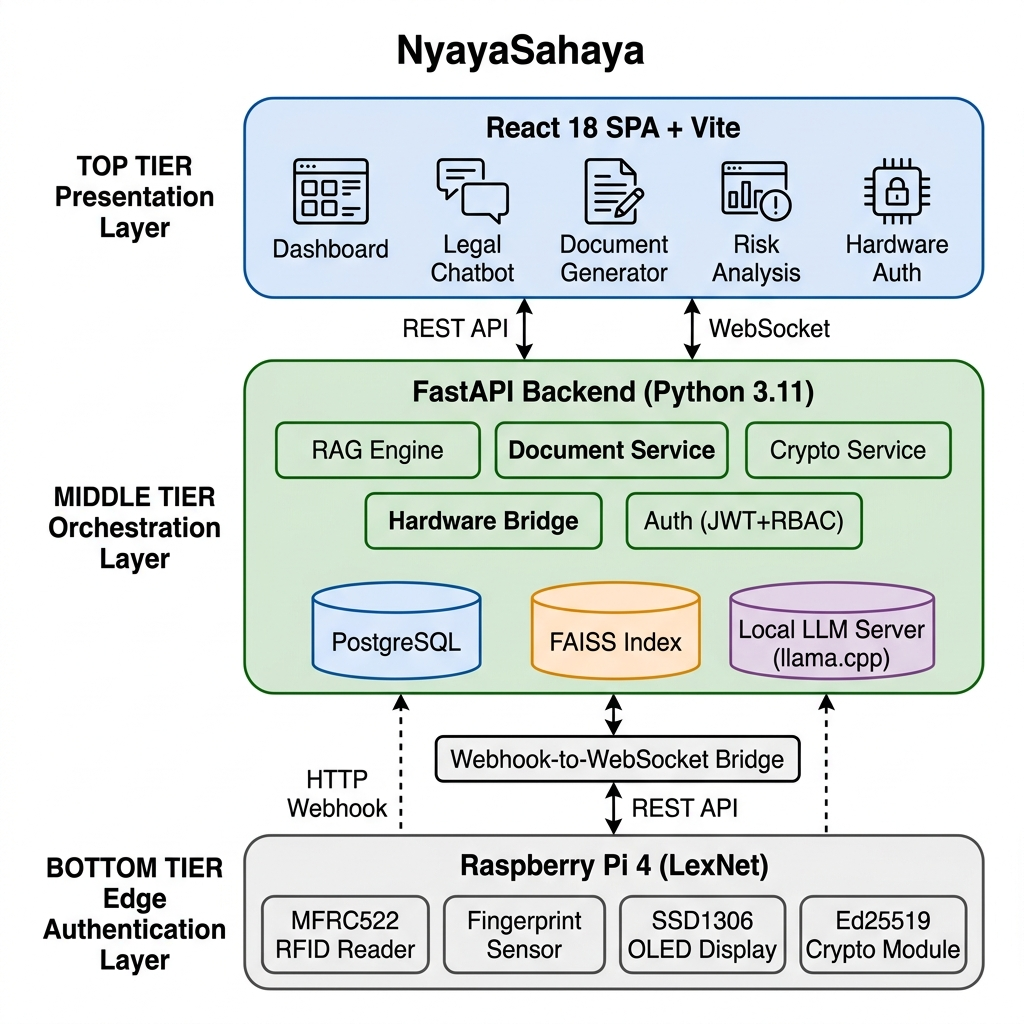
\includegraphics[width=0.70\textwidth]{figures/system_architecture.png}
\caption{Abstract system architecture of NyayaSahaya showing the presentation layer, orchestration layer, and trusted edge component, along with their high-level interactions.}
\label{fig:system_arch}
\end{figure*}

\subsection{Frontend Layer}

The presentation layer provides a guided interface for legal inquiry, document management, and verification monitoring. It emphasizes clarity, minimal steps, and consistent feedback to reduce cognitive load for non-expert users. Role-aware views present only the actions relevant to each user category while keeping sensitive controls behind appropriate permissions. The interface also surfaces explanations and next-step prompts to make complex workflows feel linear and understandable.

\subsection{Backend Orchestration Layer}

The orchestration layer coordinates retrieval, analysis, signing, and access control as cohesive services. It enforces policy boundaries, mediates requests between the interface and the trusted edge component, and maintains auditability across document workflows. The implementation is modular to support future extensions without exposing internal mechanics to the client. It also normalizes inputs and outputs to keep user-facing responses consistent even when internal processes vary.

\subsection{Edge Authentication Layer (LexNet)}

The edge authentication layer performs presence verification and emits signed assertions that can be audited by the orchestration layer. The device is treated as a trust anchor, and its responsibilities are deliberately scoped to authentication and integrity signaling. This separation prevents client-side tampering and keeps verification logic outside the presentation layer.

\subsection{Data Persistence Layer}

NyayaSahaya maintains a secure data store for users, documents, and analysis artifacts. A tamper-evident ledger records document provenance and integrity metadata, while access control policies govern sharing and visibility. This structure enables traceability of document actions without exposing sensitive internal representations.

\subsection{Communication Architecture}

Communication between tiers follows an event-driven pattern. The orchestration layer mediates edge authentication signals and exposes only sanitized status updates to the interface, ensuring that the client never communicates directly with the trusted device. This separation preserves a clean security boundary and supports real-time feedback without exposing implementation details. The flow is designed to be robust to intermittent connectivity while preserving a clear audit trail.

% =============================================================
% SECTION IV: METHODOLOGY
% =============================================================
\section{Methodology}
\label{sec:methodology}

This section outlines the high-level approach behind NyayaSahaya's core subsystems. Implementation specifics, parameters, and sensitive operational details are intentionally abstracted.

\subsection{Dual-Path Retrieval and Contextual Grounding}

NyayaSahaya uses a dual-path strategy to support both general legal questions and document-specific inquiries. A routing component selects an appropriate pathway based on the presence of document context. One path retrieves relevant legal context from a curated knowledge base, while the other focuses on the user-provided document to preserve its full contextual structure. The two paths converge into a unified response pipeline that produces grounded, user-facing guidance. Fig.~\ref{fig:rag_pipeline} provides a conceptual view of this dual-path flow.

\begin{figure*}[!t]
\centering
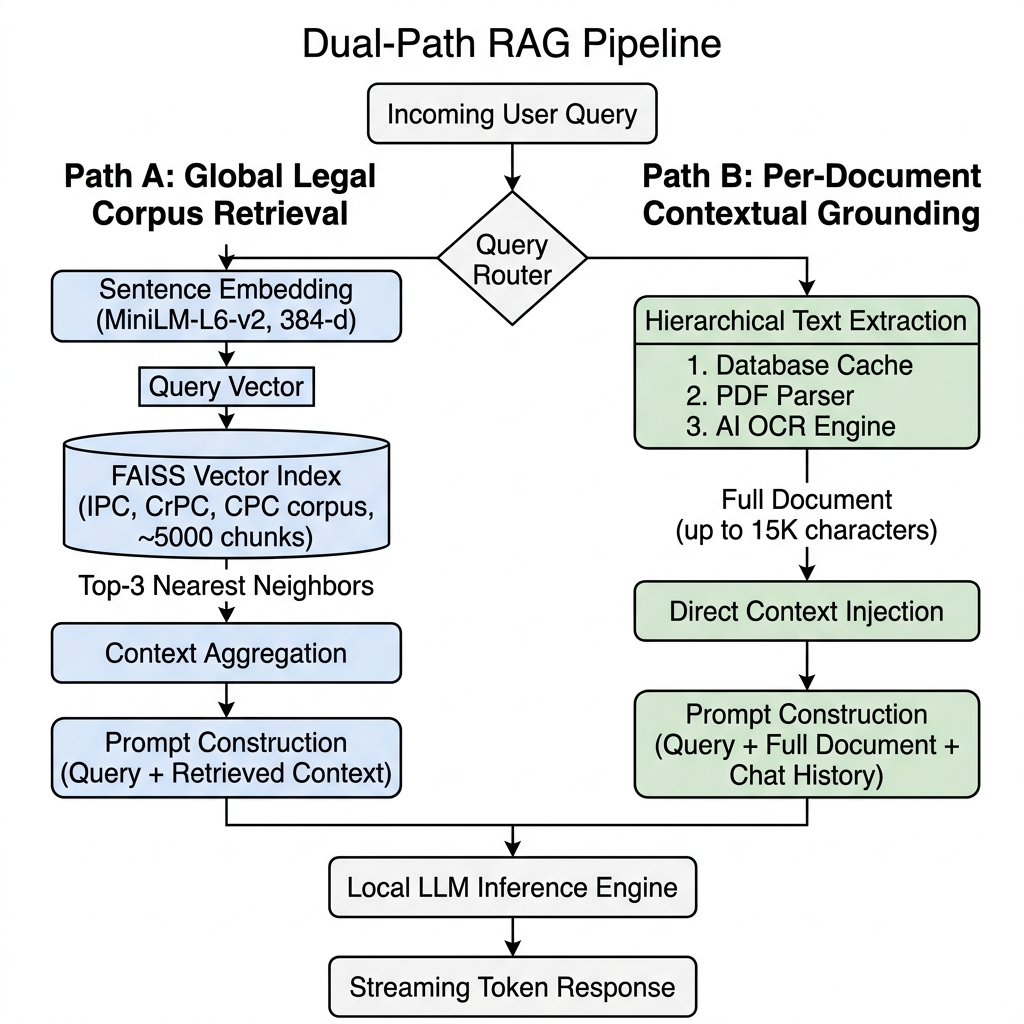
\includegraphics[width=0.70\textwidth]{figures/rag_pipeline.png}
\caption{Abstract dual-path retrieval and grounding flow. One path emphasizes global context retrieval while the other emphasizes document-specific grounding, converging into a single response pipeline.}
\label{fig:rag_pipeline}
\end{figure*}

\subsection{Authentication and Integrity}

The platform employs a trusted edge component to verify user presence and to emit signed integrity assertions. These assertions are validated by the orchestration layer and linked to document actions, enabling auditable workflows without exposing sensitive verification steps to the client interface. The resulting trust chain allows document actions to be traced to verified interactions without revealing the underlying verification mechanism.

\subsection{Document Analysis}

Document analysis produces structured summaries, key term highlights, and risk-oriented observations. The pipeline balances automated extraction with consistency checks and re-analysis triggers to avoid stale or incomplete outputs while keeping operational details confidential. Outputs are designed for practical review, emphasizing clarity and traceable rationale rather than technical internals.

% =============================================================
% SECTION V: IMPLEMENTATION
% =============================================================
\section{Implementation Details}
\label{sec:implementation}

This section summarizes the system realization at an abstract level. NyayaSahaya is implemented as a set of modular services that align with the architecture described earlier, with clear separation between the user interface, orchestration logic, and trusted edge component. The design emphasizes confidentiality, access control, and auditability, while keeping operational details and code-level specifics out of the paper.

Key implementation considerations include secure boundary enforcement between layers, consistent user experience across legal workflows, and resilient processing of document ingestion, analysis, and integrity checks. The overall design aims to balance responsiveness with trust, ensuring that sensitive operations remain isolated from the client while still providing timely feedback to users.

To support real-world legal use, the system also incorporates careful state management and error handling paths so that interruptions do not compromise document integrity or user confidence. The interface flow is structured to make verification status visible at every stage, and the orchestration layer preserves a consistent audit trail across actions. This emphasis on predictable behavior and clear feedback is central to the platform's reliability in sensitive workflows.

% =============================================================
% SECTION VI: RESULTS AND DISCUSSION
% =============================================================
\section{Evaluation Summary}
\label{sec:results}

We conducted a qualitative evaluation across the system's core capabilities, focusing on retrieval relevance, document analysis utility, authentication responsiveness, and integrity assurance. The results indicate that the dual-path retrieval strategy provides consistent, context-aware guidance for both general legal questions and document-specific queries. Document analysis outputs were judged to be coherent and useful for downstream review, and integrity checks reliably signaled tampering or mismatch conditions.

From a usability perspective, the interaction flow remained responsive and predictable, with clear status feedback across document and verification workflows. Reviewers noted that the system's structure made it easier to trace how guidance was formed and when verification steps were completed. Overall, the evaluation supports the feasibility of the proposed architecture for trustworthy legal assistance while maintaining an abstract, privacy-conscious operational footprint.

% =============================================================
% SECTION VII: CONCLUSION
% =============================================================
\section{Conclusion and Future Work}
\label{sec:conclusion}

This paper presented NyayaSahaya, a comprehensive legal assistance platform that integrates retrieval-augmented guidance, hardware-rooted authentication, and document integrity safeguards into a unified system for the Indian legal domain. The work emphasizes a clear separation between user interaction, orchestration, and trusted verification, enabling practical workflows without exposing sensitive implementation details.

The qualitative evaluation indicates that the system can provide consistent, context-aware legal assistance while maintaining privacy and trust. By abstracting the technical internals and focusing on user-centered workflows, NyayaSahaya addresses a critical gap in legal technology where usability and integrity must coexist.

\subsection{Future Directions}

Future work will explore broader language coverage, stronger governance and auditing mechanisms, and expanded document workflows that better reflect real-world legal practice. We also plan to strengthen the system's adaptability to diverse institutional requirements while preserving privacy, accountability, and trust.


\bibliographystyle{IEEEtran}
\bibliography{references}

\end{document}
